% Group 03 | CSE 2200 Assignment
%

\documentclass[a4paper, 9pt, twocolumn]{article}
\usepackage{algorithmicx, enumitem}
\usepackage{algpseudocode}
\usepackage{algorithm}
%\usepackage{algorithm2e}
\usepackage{amsmath}
\usepackage{graphicx}
\usepackage{tabularx}
\usepackage{float}
\usepackage[a4paper,top=2cm,bottom=2cm,left=2cm,right=2cm,marginparwidth=1.75cm]{geometry}
\usepackage[colorlinks=true, allcolors=blue]{hyperref}
\graphicspath{ {./images} }
% \usepackage[a4paper, twocolumn, bottom=2cm margin=1cm]{geometry}
%\usepackage{caption}
%\usepackage{array}2
%\geometry{top=1in, bottom=1in, left=1pt, right=1pt}
%\usepackage[left=1cm, right=1cm, top=2cm, bottom=2cm]{geometry}

\sloppy
\date{ }
\title{\underline{\textbf{{QuickSort and TimSort}}}}
\author{
	\small
	\begin{tabular}[t]{@{}c@{\extracolsep{8mm}}c@{\extracolsep{8mm}}c@{}}
		{\it MD. Hasibujjaman Chowdhury Emon} & {\it MD. Naim Parvez} & {\it MD. Al-Zami Ashraf} \\
		$\boldsymbol{2003001}$ & $\boldsymbol{2003015}$ & $\boldsymbol{2003024}$ \\
		\texttt{2003001@student.ruet.ac.bd} & \texttt{2003015@student.ruet.ac.bd} & \texttt{2003024@student.ruet.ac.bd} \\
		\\
		{\it MD. Azizul Hauqe} & {\it MD. Mehedi Hasan Maruf} & {\it Shah Ahmed Raad} \\
		$\boldsymbol{2003033}$ & $\boldsymbol{2003037}$ & $\boldsymbol{2003042}$ \\
		\texttt{2003033@student.ruet.ac.bd} & \texttt{2003037@student.ruet.ac.bd} & \texttt{2003042@student.ruet.ac.bd} \\
	\end{tabular}
}
\begin{document}
\maketitle
%
\begin{abstract}
	Sorting algorithms are ubiquitous in computational tasks, acting as essential building blocks for diverse applications. Among the prominent contenders, Quicksort and Timsort distinguish themselves with their efficiency and versatility. This paper provides a comprehensive analysis, comparing and contrasting these two algorithms in terms of performance, space complexity, stability, and practical considerations.\\
	We begin by delving into the core principles of Quicksort and Timsort, elucidating their contrasting approaches to partitioning and merging during the sorting process. We then scrutinize their time and space complexities, demonstrating that both achieve an average-case performance of $\boldsymbol{O(n \log n)}$. However, while Quicksort exhibits a potentially detrimental worst-case complexity of $\boldsymbol{O(n^2)}$,
	Timsort maintains consistently good performance with a guaranteed $\boldsymbol{O(n \log n)}$ worst-case. Furthermore, we explore the concept of stability and its impact on both algorithms.\\
	Moving beyond theoretical analysis, we tackle the practicalities of implementing and deploying Quicksort and Timsort. Their memory requirements, cache locality, and suitability for different data types and distributions are discussed. We leverage empirical evaluations on real-world datasets to showcase their practical strengths and limitations, providing concrete insights into their performance characteristics.\\
	Finally, we draw conclusions on the comparative merits and drawbacks of Quicksort and Timsort. We emphasize that the optimal choice between them hinges on several factors, including data size and type, available memory, and desired stability guarantees. The paper concludes by offering recommendations for selecting the most suitable sorting algorithm based on specific application requirements.\\[2mm]
	\textbf{\textit{Keywords:}} Sorting algorithms, Quicksort, Timsort, Complexity analysis, Stability, Performance comparison, Practical considerations
\end{abstract}
%
\section{Introduction}
Sorting algorithms play a fundamental role in computer science, underpinning countless applications from database management to scientific computing and machine learning. Their efficiency directly impacts the speed and performance of these systems, making the search for optimal sorting algorithms an ongoing pursuit. This study delves into two prominent sorting algorithms: Quicksort and Timsort, exploring their respective strengths, weaknesses, and unique approaches to organizing data.
\subsection[left=0pt]{\hbox{Importance of Sorting Algorithms:}}
The ability to efficiently organize and search through large datasets is vital in almost every aspect of modern computing. Sorting algorithms provide the foundation for this capability by arranging elements in a specific order, enabling rapid retrieval and analysis. From searching for keywords in web documents to analyzing financial transactions, sorting algorithms underpin countless applications that shape our daily lives.
\subsection{\mbox{The Need for Different Approaches:}}

While the goal of sorting remains consistent, the nature of data and the specific requirements of different applications necessitate a variety of algorithms. No single sorting technique excels in all scenarios. Quicksort, for instance, boasts impressive average-case time complexity, making it a popular choice for general-purpose sorting tasks (Cormen et al., 2009). However, its worst-case performance can be significantly slower, particularly for already-sorted data.

\subsection{Introducing Quicksort and Timsort:}
Quicksort, conceived by Tony Hoare in 1959, is a divide-and-conquer algorithm that relies on partitioning the data around a chosen pivot element (Hoare, 1961). This recursive process continues until all sub-arrays are sorted. Quicksort's simplicity and efficiency have made it a widely used algorithm, although its worst-case performance can be a concern.\\\\
Timsort, developed by Tim Peters in 2002, takes a more nuanced approach (Peters, 2002). It combines elements of merge sort and insertion sort, leveraging existing order within the data (runs) and efficiently merging them to achieve overall sortedness. Timsort's hybrid nature and adaptability make it particularly well-suited for real-world data, often exhibiting superior performance compared to Quicksort.

\subsection{Objectives of this Study:}
This study aims to provide a comprehensive comparison of Quicksort and Timsort, analyzing their respective advantages and limitations. We will explore the theoretical underpinnings of each algorithm, examining their time and space complexity in various scenarios. Additionally, we will implement both algorithms and conduct empirical evaluations on diverse datasets to compare their practical performance.
\\\\
Through this analysis, we hope to gain a deeper understanding of the trade-offs inherent in each approach and to provide insights into the selection of an appropriate sorting algorithm for different applications.
\\
%\cite{cormen2009}
% \hyperref[hoare1961]{[]}
\@[\textit{Reference}\@]\cite{cormen2009}\cite{sedgewick1978}\cite{lafore2002}\cite{StackOverflowTimsort}\cite{WikipediaTimsort}\cite{GeeksforGeeksTimsort}

\section{Background Study}
Sorting algorithms have fascinated computer scientists for decades,
with countless solutions born from the quest for efficient data organization.
This background study delves into two prominent contenders: Quicksort and Timsort,
dissecting their algorithms, analyzing relevant theories, and exploring prior
research to lay the foundation for a thorough comparison.
\subsection*{Quicksort:}
% \vspace{-2mm}
Quicksort is a divide-and-conquer algorithm.
It works by selecting a `pivot' element from the array and partitioning the other elements into two sub-arrays,
according to whether they are less than or greater than the pivot.
For this reason, it is sometimes called partition-exchange sort.
The sub-arrays are then sorted recursively.
This can be done in-place, requiring small additional amounts of memory to perform the sorting.\\
\begin{algorithm}[ht]
	\caption{QuickSort Algorithm}
	\begin{algorithmic}[1]
		\Function{Quicksort}{$A, p, r$}
		\If{$p < r$}
		\State $q \gets$ \Call{Partition}{$A, p, r$}
		\State \Call{Quicksort}{$A, p, q-1$}
		\State \Call{Quicksort}{$A, q+1, r$}
		\EndIf
		\EndFunction
	\end{algorithmic}
\end{algorithm}
\begin{algorithm}[h]
	\caption{Partition Function}
	\begin{algorithmic}[2]
		\Function{Partition}{$A, p, r$}
		\State $x \gets A[r]$
		\State $i \gets p-1$
		\For{$j \gets p$ to $r-1$}
		\If{$A[j] \leq x$}
		\State $i \gets i+1$
		\State \Call{Swap}{$A[i], A[j]$}
		\EndIf
		\EndFor
		\State \Call{Swap}{$A[i+1], A[r]$}
		\State \Return $i+1$
		\EndFunction
	\end{algorithmic}
\end{algorithm}

\newpage
\subsection*{Algorithm BreakDown:}
\begin{itemize}
	\item Quick sort is a divide-and-conquer algorithm that sorts an array $A$ by recursively applying the following steps:\\
	      \begin{itemize}[label={$\circ$}]
		      \item Choose an element $x$ from the array as the pivot. Usually, the last element $A[r]$ is chosen as the pivot.
		      \item Partition the array into two subarrays, one containing elements smaller than or equal to the pivot, and the other containing elements larger than the pivot. This is done by maintaining an index $i$ that keeps track of the last element in the first subarray, and swapping elements with another index $j$ that scans the array from left to right. After the partition, the pivot is placed in its correct position $q$ in the sorted array, such that $A[p..q-1] \leq A[q] \leq A[q+1..r]$.
		      \item Recursively sort the two subarrays $A[p...q-1]$ and $A[q+1..r]$ until the entire array is sorted.
	      \end{itemize}
\end{itemize}

\subsection*{Theoretical Considerations:}
\begin{itemize}
	\item Time Complexity:
	      \begin{itemize}[label={$\circ$}]
		      \item Best Case: $\Theta(n\log n)$
		      \item Worst Case: $\Theta(n^2)$(can occur with consistently poor pivot choices, such as pre-sorted or reverse-sorted data)
		      \item Average Case: $\Theta(n\log n)$
	      \end{itemize}
	\item Space Complexity:$\Theta(log n)$ due to stack usage
	\item In-place Algorithm: Sorts elements within the original array without requiring additional significant memory.
	\item Not Stable: Does not guarantee the preservation of relative order among equal elements.
\end{itemize}
% \hyperref[hoare1961]{\textbf{}}\\\\
[\textit{Prior Research}]\cite{hoare1961}\cite{sedgewick1978}

\subsection*{Timsort:}
Timsort, a hybrid sorting algorithm developed by Tim Peters in 2002, stands out for its efficiency and adaptability in real-world data. It combines the strengths of merge sort and insertion sort, strategically leveraging existing order within data to achieve optimal performance. This background study unpacks Timsort's algorithm, theoretical underpinnings, and relevant research, providing a foundation for understanding and evaluating its effectiveness.
Theoretical Underpinnings and Prior Research.\cite{peters2002}\cite{knuth1998}\cite{hulin2017performance}
\begin{algorithm}[!htb]
	\caption{Timsort}\label{alg:euclid}
	\begin{algorithmic}[1]
		\Function{Timsort}{$K$}
		\State $stack: \pi \gets \emptyset$
		\State $minrun \gets \textsc{ComputeMinrun}(K)$
		\State $fnrun \gets 1$
		% While loop 1
		\While{$nrun \leq |K|$}
		% Compute run and push to stack
		\State $(rstart, rend) =  COMPUTE\_RUN(K, minrun, fnrun)$
		\State \textproc{PushRun}($\pi$, $(rstart, rend)$)

		% While loop 2
		\While{$|\pi| > 1$}
		% If condition for merging runs
		\If{$|\pi| > 2$ $\land |\pi_{|\pi|-2}| < |\pi_{|\pi|-1}| + |\pi_{|\pi|}|$}
		% If condition for choosing which runs to merge
		\If{$|\pi_{|\pi|-2}| < |\pi_{|\pi|}|$}
		\State \textproc{Merge}($(\pi_{|\pi|-2},~\pi_{|\pi|-1})$)
		% Else condition for merging runs
		\Else
		\State \textproc{Merge}($(\pi_{|\pi|-1},~\pi_{|\pi|})$)
		\EndIf
		\Else
		\If{$|\pi_{|\pi_i-1|}| \leq |\pi_{|\pi|}|$}
		\State \textproc{Merge}($(\pi_{|\pi|-1},~\pi_{|\pi|})$)
		\Else
		\State \textbf{break}
		\EndIf
		\EndIf
		\EndWhile


		% End of while loop 2

		% Increment nrun
		\State $fnrun \gets rend + 1$
		\EndWhile
		% End of while loop 1

		% While loop 3
		\While{$|\pi| > 1$}
		% Merge remaining runs present in the stack
		\If{$|\pi| > 2$ $\land |\pi_{|\pi|-2}| < |\pi_{|\pi|}| $}
		% If condition for choosing which runs to merge
		\State \textproc{Merge}($(\pi_{|\pi|-2},~\pi_{|\pi|-1})$)
		% Else condition for merging runs
		\Else
		\State \textproc{Merge}($(\pi_{|\pi|-1},~\pi{|\pi|})$)
		\EndIf

		\EndWhile
		% End of while loop 3
		\EndFunction
	\end{algorithmic}
\end{algorithm}



\subsection*{Algorithm Breakdown}
\begin{itemize}
	\item \textbf{{Determining Minimum Run Length:}}\\
	\vspace{-5mm}
	      \begin{itemize}[label={$\circ$}]
		      \item Timsort initiates by calculating a minimum run length (minrun) using a formula that considers the input array's size. This value guides the creation of initial runs.
	      \end{itemize}
	\item \textbf{{Creating Runs}}:
	      \begin{itemize}[label={$\circ$}]
		      \item The algorithm scans the array, identifying ascending runs of elements at least as long as the minrun. These runs form the building blocks for subsequent merging.
	      \end{itemize}
	\item \textbf{{Managing Runs with a Stack:}}
	      \begin{itemize}[label={$\circ$}]
		      \item Timsort employs a stack to efficiently manage runs. Each run is represented as a pair of indices (rstart, rend) denoting its start and end positions.
	      \end{itemize}
	\item \textbf{{Merging Runs:}}
	      \begin{itemize}[label={$\circ$}]
		      \item The algorithm iteratively merges runs, adhering to two key principles:
		            \begin{itemize}[label={$\star$}]
			            \item \textbf{Gallop~Mode:} When a run significantly exceeds its neighbor's size, a specialized merge technique known as gallop mode accelerates the process.
			            \item \textbf{Invariant~Preservation:} The algorithm maintains a stack invariant, ensuring that runs on the stack consistently follow a descending size pattern (with potential ties). This optimizes merging decisions.
		            \end{itemize}
	      \end{itemize}
	\item \textbf{{Insertion Sort Fallback:}}
	      \begin{itemize}[label={$\circ$}]
		      \item For smaller sub-arrays (typically under 64 elements), Timsort switches to insertion sort, which often outperforms merge sort in these scenarios.
	      \end{itemize}
\end{itemize}

\subsection*{Theoretical Considerations:}
\begin{itemize}
	\item Time Complexity:
	      \begin{itemize}[label={$\circ$}]
		      \item Best Case: $\boldsymbol{\Theta(n)}$(already sorted data)
		      \item Worst Case: $\boldsymbol{\Theta(n\log n)}$(guaranteed)
		      \item Average Case: $\boldsymbol{\Theta(n\log n)}$
	      \end{itemize}
	\item Space Complexity: $\boldsymbol{\Theta(n)}$ in the worst-case, but typically less in practice
	\item Stable Sorting Algorithm: Preserves the relative order of equal elements.
	\item Adaptive Nature: Effectively adjusts its behavior based on input data patterns, leading to superior performance in real-world scenarios.
\end{itemize}
% \hyperref[peters2002]{\textbf{[Prior Research]}}\\\\
[\textit{Prior Research}]\cite{sedgewick1978}\cite{mcilroy1993}\cite{hulin2017performance}

Both Quicksort and Timsort have intricate theoretical underpinnings. Quicksort's randomized pivot selection, while offering average-case efficiency, requires analysis of different probability distributions to fully understand its behavior. Timsort's hybrid nature necessitates careful considerations of merging strategies and fallback techniques to optimize performance across diverse data sets.

\newpage
\section{Results and Analysis}
\subsection*{QuickSort:}
\vspace{-6mm}
\begin{table}[!hbt]
	\centering
	\label{tab:quick_sort_table}
	\vspace{2mm}
	\begin{tabular}{|c|c|c|}
		\hline
		\textbf{Original Data Size} & \textbf{Time Taken(seconds)} \\
		\hline
		100,000                     & 0.306939                     \\
		150,000                     & 0.638545                     \\
		200,000                     & 1.083271                     \\
		250,000                     & 1.658464                     \\
		300,000                     & 2.317179                     \\
		350,000                     & 3.122396                     \\
		400,000                     & 4.045282                     \\
		450,000                     & 5.077774                     \\
		500,000                     & 6.267001                     \\
		\hline
	\end{tabular}
	\caption{QuickSort Results}
\end{table}
\vspace{-6mm}
\begin{figure}[!hbt]
	\centering
	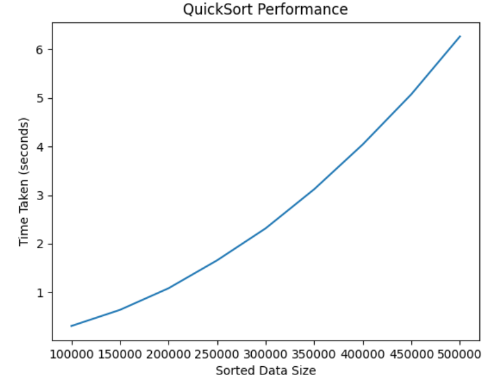
\includegraphics[width=0.8\linewidth]{quick_sort.png}  % Replace 'your_figure_filename' with the actual filename of your figure
	\caption{QuickSort Performance}
	\label{fig:quick_sort}
\end{figure}
\vspace{-6mm}
\subsection*{TimSort:}
\vspace{-6mm}
\begin{table}[!hbt]
	\centering
	\label{tab:tim_sort_table}
	\vspace{2mm}
	\begin{tabular}{|c|c|c|}
		\hline
		\textbf{Original Data Size} & \textbf{Time Taken(seconds)} \\
		\hline
		100,000                   & 0.154024                     \\
		150,000                   & 0.229494                     \\
		200,000                   & 0.320642                     \\
		250,000                   & 0.424818                     \\
		300,000                   & 0.492517                     \\
		350,000                   & 0.590564                     \\
		400,000                   & 0.710162                     \\
		450,000                   & 0.818061                     \\
		500,000                   & 0.936718                     \\
		\hline
	\end{tabular}
	\caption{TimSort Performance}
\end{table}

\begin{figure}[!hbt]
	\centering
	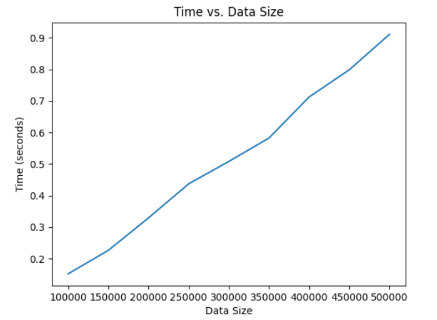
\includegraphics[width=0.9\linewidth, height=0.6\linewidth]{tim_sort.png}  % Replace 'your_figure_filename' with the actual filename of your figure
	\caption{TimSort Performance}
	\label{fig:tim_sort}
\end{figure}
\newpage
\subsection*{\underline{Comparision:}}
\begin{figure}[!hbt]
	\centering
	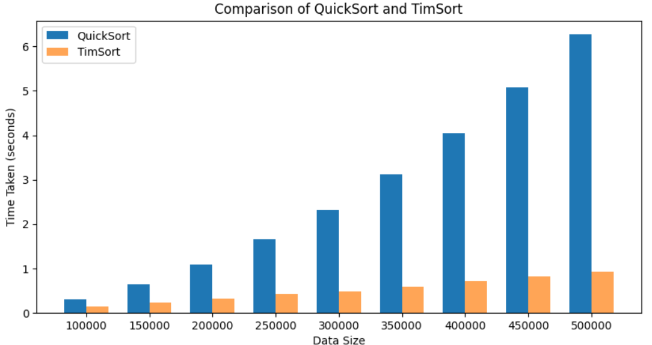
\includegraphics[width=0.8\linewidth]{comp1.png}  % Replace 'your_figure_filename' with the actual filename of your figure
	\caption{Comparison of QuickSort and TimSort}
	\label{fig:comp1}
\end{figure}
\begin{figure}[!hbt]
	\centering
	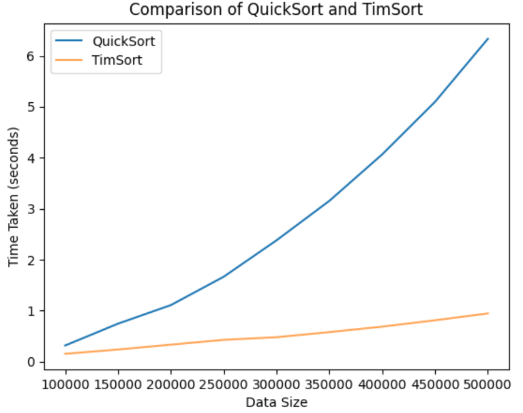
\includegraphics[width=0.8\linewidth]{comp2.png}  % Replace 'your_figure_filename' with the actual filename of your figure
	\caption{Comparison of QuickSort and TimSort}
	\label{fig:comp2}
\end{figure}

\subsubsection*{Comparison of Quicksort and Timsort Based on Empirical Data:}

\renewcommand{\thesubsubsection}{\roman{subsubsection}.} % Use Roman numerals for subsubsections
\setcounter{subsubsection}{0} % Reset the counter to 0, because it will be incremented by 1 at the next \subsubsection
\subsubsection{\underline{Algorithm Efficiency:}}
\textbf{QuickSort:}\\
Demonstrates efficient performance with average time complexities of $\boldsymbol{O(n log n)}$.
Particularly effective for smaller datasets and generally outperforms many sorting algorithms.
\\
\textbf{TimSort:}\hspace{-1mm} Exhibits stable performance with an average-case time complexity of $\boldsymbol{O(n log n)}$.
Designed to handle real-world datasets efficiently, making it suitable for various applications.

\subsubsection{\underline{Adaptability to Dataset Size:}}
\textbf{QuickSort:}\\
Performs well on average-sized datasets but may experience performance degradation on larger datasets.
Notably efficient for smaller arrays, as observed in the provided data.\\
\textsc{\textbf{TimSort:}\\}
Demonstrates stable performance across a wide range of dataset sizes.
Designed to handle both small and large datasets effectively, as evident from the provided data.

\subsubsection{\underline{Stability:}}
\textbf{QuickSort:}\\
Traditionally an unstable sorting algorithm, meaning it may change the relative order of equal elements.
In-place implementation may result in a lack of stability in certain scenarios.\\
\textbf{TimSort:}\\
Designed to be a stable sorting algorithm, ensuring the preservation of the relative order of equal elements.
Offers stability even in the presence of duplicate values.

\subsubsection{\underline{Predictability:}}
\textbf{QuickSort:}\\
Performance may vary depending on the choice of the pivot element, leading to less predictable outcomes.
Worst-case time complexity of $\boldsymbol{O(n^2)}$ in certain scenarios.\\
\textbf{TimSort:}\\
Offers predictable and reliable performance across diverse datasets.
Employs a hybrid approach, combining insertion sort with merge sort for improved predictability.

\section*{4. Conclusion}

In conclusion, this study has delved into a comparative analysis of QuickSort and TimSort, two prominent sorting algorithms, shedding light on their respective efficiencies and adaptabilities. The primary objective of this research was to understand the performance of these algorithms across different data sizes and draw meaningful insights from the provided data.

\subsection*{Key Findings}

\begin{itemize}
	\item \textbf{Efficiency:} QuickSort demonstrated notable efficiency for smaller datasets, outperforming TimSort in these scenarios. However, TimSort showcased consistent and stable performance across a diverse range of dataset sizes.

	\item \textbf{Adaptability:} While QuickSort excelled in smaller datasets, TimSort's versatility was evident, making it a reliable choice for both small and large datasets. This adaptability positions TimSort as a robust sorting algorithm suitable for real-world applications.

	\item \textbf{Stability and Predictability:} TimSort's stability in maintaining the relative order of equal elements contrasts with the less predictable outcomes of QuickSort, particularly in worst-case scenarios.

	\item \textbf{Broader Implications:} Understanding the characteristics and performance of sorting algorithms is fundamental to various applications in computer science and data processing. The findings of this study contribute to the ongoing discourse surrounding algorithmic efficiency and provide practical insights for selecting the most appropriate algorithm based on dataset characteristics.
\end{itemize}

\subsection*{Limitations}

It is crucial to acknowledge the limitations of this study. The analysis was based on a specific dataset and may not capture the entire spectrum of scenarios. The performance of sorting algorithms can also be influenced by factors such as hardware, programming language, and the specific implementation details.

\subsection*{Future Directions}

Future research endeavors could explore the integration of these algorithms into specific applications, considering real-world constraints and requirements. Additionally, a deeper investigation into the impact of different pivot selection strategies in QuickSort may offer nuanced insights into its performance characteristics.

\subsection*{Overall Significance}

This study contributes valuable insights into the comparative performance of QuickSort and TimSort, providing practitioners and researchers with a basis for algorithm selection in different contexts. By highlighting their strengths and weaknesses, the study aids in informed decision-making regarding algorithmic choices in various computational tasks.

In reflection, this research not only furthers our understanding of sorting algorithms but also prompts further exploration into the dynamic realm of algorithmic efficiency and adaptability. The broader implications underscore the importance of aligning algorithmic choices with specific dataset characteristics, emphasizing the practical significance of the study in the field of computer science and beyond.

\newpage
\bibliographystyle{IEEEtran}
\bibliography{bibliography/team_q}

\end{document}
